\subsection {TopLevel}
\label{sec:TopLevel}
\sbol{TopLevel} is an abstract class that is extended by any \sbol{Identified} class that can be found at the top level of an SBOL document or file. In other words, \sbol{TopLevel} objects are not nested inside any other object via a composite aggregation or black diamond arrow association property. Instead of nesting, composite \sbol{TopLevel} objects refer to subordinate \sbol{TopLevel} objects by their \sbol{URI}s using shared aggregation or white diamond arrow association properties. The \sbol{TopLevel} classes defined in this specification are \sbol{Sequence}, \sbol{Component}, \sbol{Model}, \sbol{Collection}, \sbol{CombinatorialDerivation}, \sbol{Implementation}, \sbol{Attachment}, \sbol{ExperimentData}, \sbol{Experiment}, (\ref{uml:toplevel}).


\begin{figure}[ht]
\begin{center}
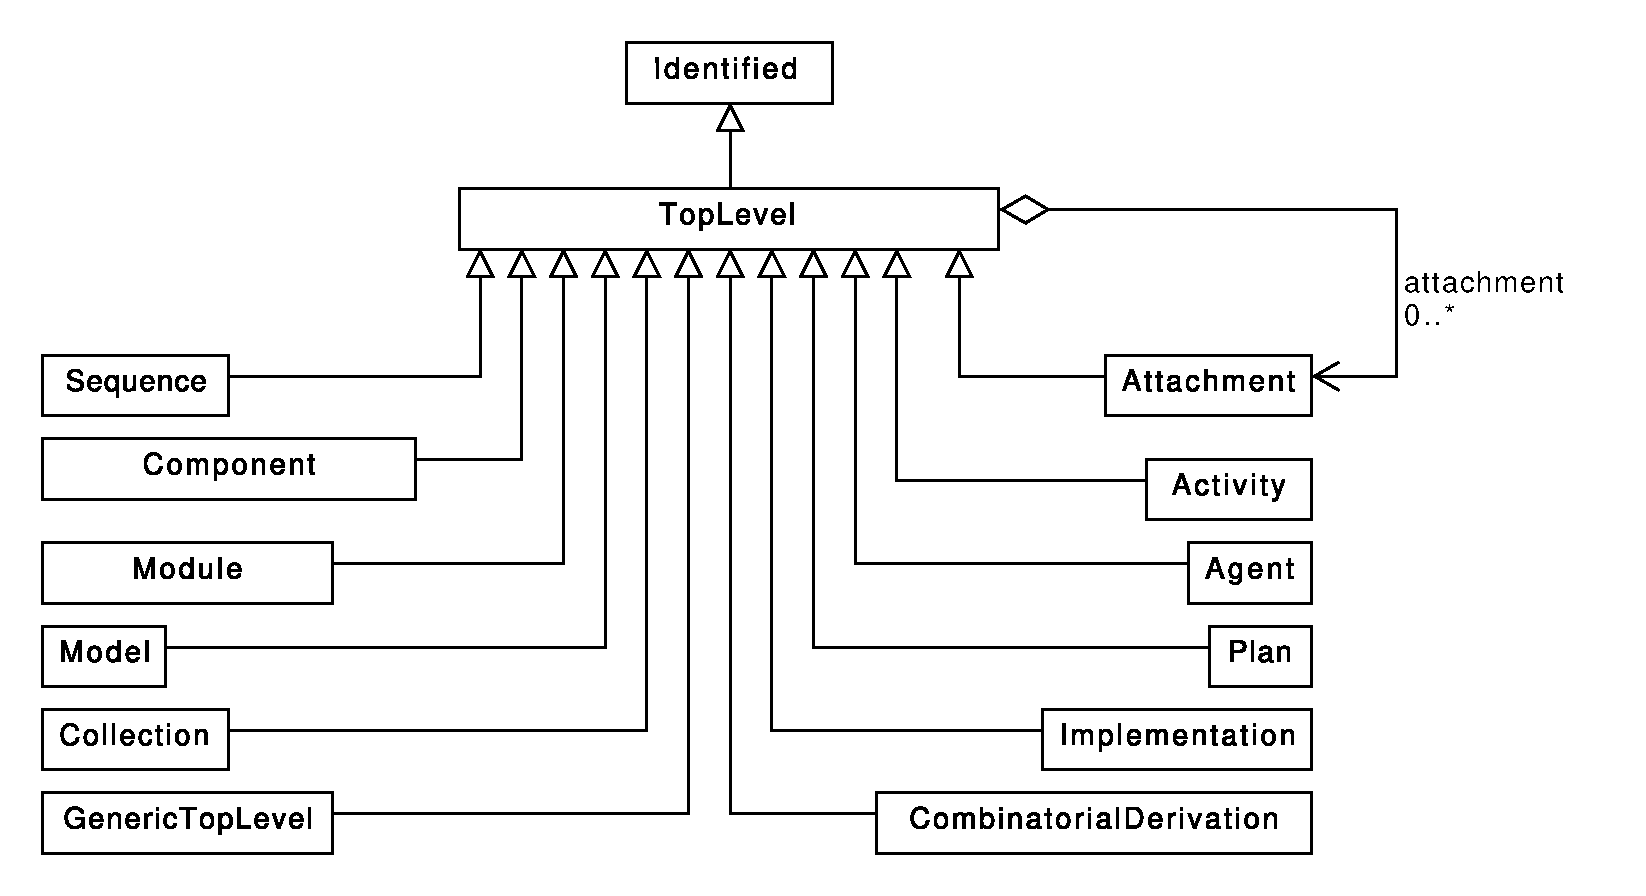
\includegraphics[width=\textwidth]{uml/toplevel}
\caption[]{Classes that inherit from the \sbol{TopLevel} abstract class.}
\label{uml:toplevel}
\end{center}
\end{figure}


\subparagraph{The hasAttachment property}
\label{sec:hasAttachment}
A \sbol{TopLevel} object can have zero or more \sbol{hasAttachment} properties, each of type URI specifying an \sbol{Attachment} object. The \sbol{Attachment} class is described in more detail in Section~\ref{sec:Attachment}.

